

\subsection{DeepmindLab navigation challenge}
We propose a 4-stage benchmark for reinforcement learning based methods to address the navigation problem.
While there already exists optimal algorithms to find shortest path between two points and perform optimal navigation between given set of points in a given map, the advantage of Deep reinforcement learning comes from its ability to extract required features from the input images and its promise
optimize mapping and path planning in end-to-end fashion. 
Thus we need to either integrate existing path planning and mapping methods with deep learning methods to perform end-to-end training or extend deep learning methods to learn path planning and mapping.

\begin{description}
  \ditem{Evaluate on training map, static goal location, static spawn location}
  \label{prob:sss}
   This is the easiest variation of our experiments. To perform
   optimally on this experiment, the agent needs to find and learn the
   shortest path at train time and repeat that during evaluation time.
  \ditem{Evaluate on training map, static goal location, random spawn location}
  This is a textbook version of reinforcement learning problem, especially in gridworld \cite{SuBaBOOK1998}, except we have partially observable world in form of first person view only.
  This problem is more difficult than Problem~\ref{prob:sss} because the agent
  needs to find optimal policy from each possible starting point in the maze.
  \ditem{Evaluate on training map, random goal location, static spawn location}
  Since the goal position is unknown in every episode, the agent needs to explore the maze to find the goal for the first time. Recall that the agent is respawned every time it hits the goal.
  In this case the respawning happens at a static location, and if the agent remembers the location of the map, it should be able to find the goal faster than
  the first iteration.
  Following \cite{MiPaViICLR2017}, we report the ratio
  of time taken to hit the goal first time (exploration time) vs the average of the time taken to hit goal subsequently (exploitation time). The metric is henceforth called \LatencyOneGtOne
  If this ratio is greater than 1, then we say that the agent is doing better than random path planning.
  \ditem{Evaluate on training maps with random goal location, random spawn location}
    This is the problem that is addressed by \cite{MiPaViICLR2017}
    with limited success. They evaluate this case on two maps and report \LatencyOneGtOne to be greater than 1 in one of the two maps. We evaluate the same metric on their map and ten other maps.
  \ditem{Evaluate on unseen maps, random goal, random spawn}
    Any proposed algorithms on navigation problems, should be evaluated on unseen maps.
    To our knowledge, this is the first paper to evaluate Deep reinforcement learning agents on unseen maps.
\end{description}

We also evaluate the algorithm on a few qualitative maps other than I-maze. These maps are specifically designed to query what percentage of times does the agent takes shortest path.

\setcounter{Benchmark}{0}
\begin{description}
    \ditem{Wrench map}
    This map is shown on the top row, extreme right column in Fig~\ref{fig:environments}. It has one loop and a corridor.
    The goal is placed asymmetrically in the loop and the agent is spawned in the corridor.
    Because of asymmetrical placement of the goal, one of the path to the goal is shorter than the other and there are only two possible paths.
    We record the path taken each time. If the agent has learned a greedy strategy, then it would repeat the path taken for the first time.
    We evaluate the fraction of times, the agent repeats the first path. A higher number indicates a greedy strategy.
    In second evaluation, we let the agent explore randomly untill it hits the goal via the shorterst path.
    At this point we evaluate the  fraction of times shortest path is taken. For this score 
    \ditem{Goal map}
    This map is shown on the bottom row, extreme right column in Fig~\ref{fig:environments}.
    We chose this map because this is the simplest map with a fork. Making the map any simpler will make the map homeomorphic to a straight line. 
    We evaluate the number of times the agent takes the right descision at the fork after exploring the goal once.
\end{description}

\begin{figure}%
 \vspace{-3em}%
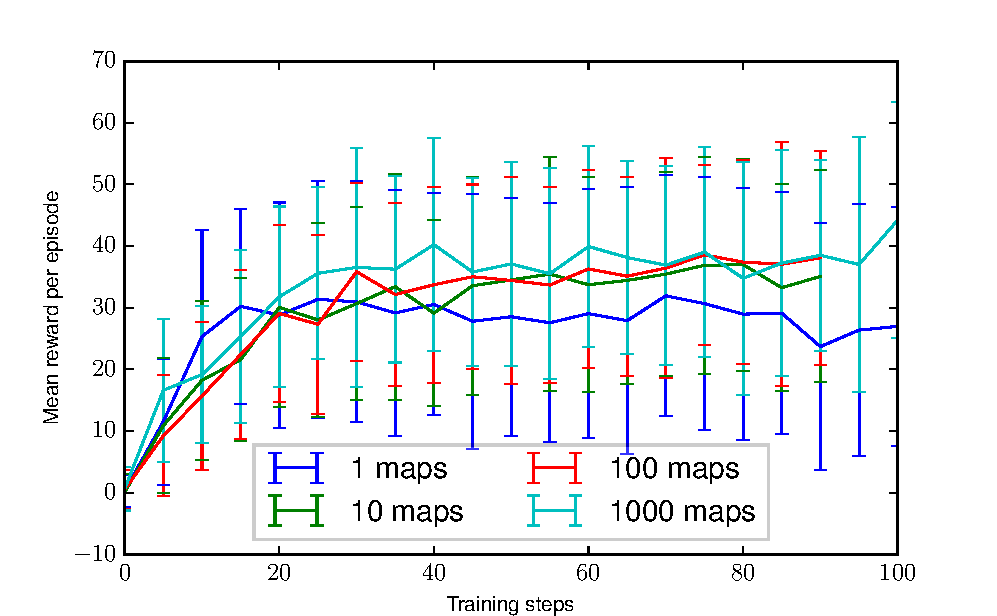
\includegraphics[width=0.5\columnwidth]{images/plot_reward_3D-1000.pdf}%
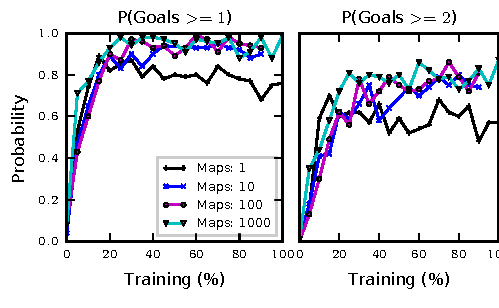
\includegraphics[width=0.5\columnwidth]{images/plot_probability_3D-1000.pdf}%
\vspace{-1em}%
\caption{Mean reward while tested on 100 unseen maps, while being trained on different number of training maps. Note that while training on 1000 maps eventually achieves high reward, it is only higher mean reward (44.2), training on 1 map hits the maximum (31) much faster.}%
\label{fig:plot_reward_on_testing}%
\end{figure}
